\section{Bibliography Review}
\label{sec:bibliography-review}

A bibliographical research was performed to determine the state of the art in the field of the project, both in terms of the models and algorithms used as well as the chosen and best-performing state and action spaces, with regard to realistic environment simulations, and the use of reinforcement learning techniques. The search was made using the “Web of Science” repository, covering the last 5 years, with the following search key:

\begin{verbatim}
    ("reinforcement learning" OR "dynamic programming" OR
     "optimal control" OR "control theory" OR "machine learning")
    AND
    ("market making" OR "market maker")
\end{verbatim}

Initially, 64 references were selected and deemed relevant to the project, with 23 of them being selected for further analysis and effectively used in our analysis,
with 4 of them being added to the list after the initial selection.
The references were selected based on their relevance to the project and tagged according to the following groups (for each non-binary category, combinations of tags were allowed):
type of data (simulated or real-time connections);
chosen state space (tensors of bid-ask spreads, order imbalance, and N-depth order books);
chosen action space (limit orders, market orders, and others); reward space (spread, volume, profit, and others);
algorithms used (Q-Learning, Deep Q-Learning, Actor-Critic, or others); whether using a multi-agent approach (dueling or market agents);
the use of model-free environments; and chosen metrics (Sharpe Ratio, PnL, and others);
finally, results were tagged by benchmarking (against other models or strategies).

State-of-the-art methodologies defined state spaces based on market-level observations, such as inventory, bid-ask spreads, and order book depths,
which align well with the real-time data available to market-making agents \cite{he2023integrating, bakshaev2020marketmaking}.
Action spaces are typically designed to include price adjustments, order placements, and cancellations,
reflecting the dynamic nature of market interactions \cite{sun2020marketmaking, gasperov2021marketmaking}.
Reward structures are tailored to balance profitability, risk, and liquidity provision,
often incorporating penalties for inventory imbalances or adverse market impacts \cite{sun2020marketmaking, gasperov2021marketmaking}.

Recent trends in reinforcement learning research emphasize model-free approaches, particularly Deep Q-Learning and Actor-Critic methods,
which leverage neural networks to approximate value functions or policies in high-dimensional spaces \cite{patel2018optimizing, ganesh2019reinforcement}.
These algorithms demonstrate strong adaptability to evolving market conditions while maintaining computational feasibility.
However, the inclusion of constraints, such as inventory and volatility penalties,
is essential to ensure practical applicability and risk management in live trading scenarios \cite{jerome2022modelbased, selser2021optimal}.

Multi-agent frameworks have also gained attention, enabling the simulation of competitive market environments where agents adapt their strategies in response to others.
These frameworks are particularly useful for studying market impact and stability under varying conditions \cite{ganesh2019reinforcement, jericevich2021simulation}.
Metrics such as the Sharpe Ratio and profit-and-loss analysis remain key benchmarks for evaluating the performance of these algorithms,
providing a robust basis for comparing different strategies \cite{bakshaev2020marketmaking, he2023integrating}.

In summary, the bibliographical review underscores the relevance of reinforcement learning in optimizing market-making strategies,
particularly when combined with realistic state, action, and reward spaces.
The insights gained from this review inform the design of our proposed restrictions-based RL framework,
which seeks to enhance the stability and interpretability of market-making algorithms while addressing critical risk management challenges.

\subsection{State, Action, and Reward Spaces}
% graph: images/state_space.png
\begin{figure}[H]
    \centering
    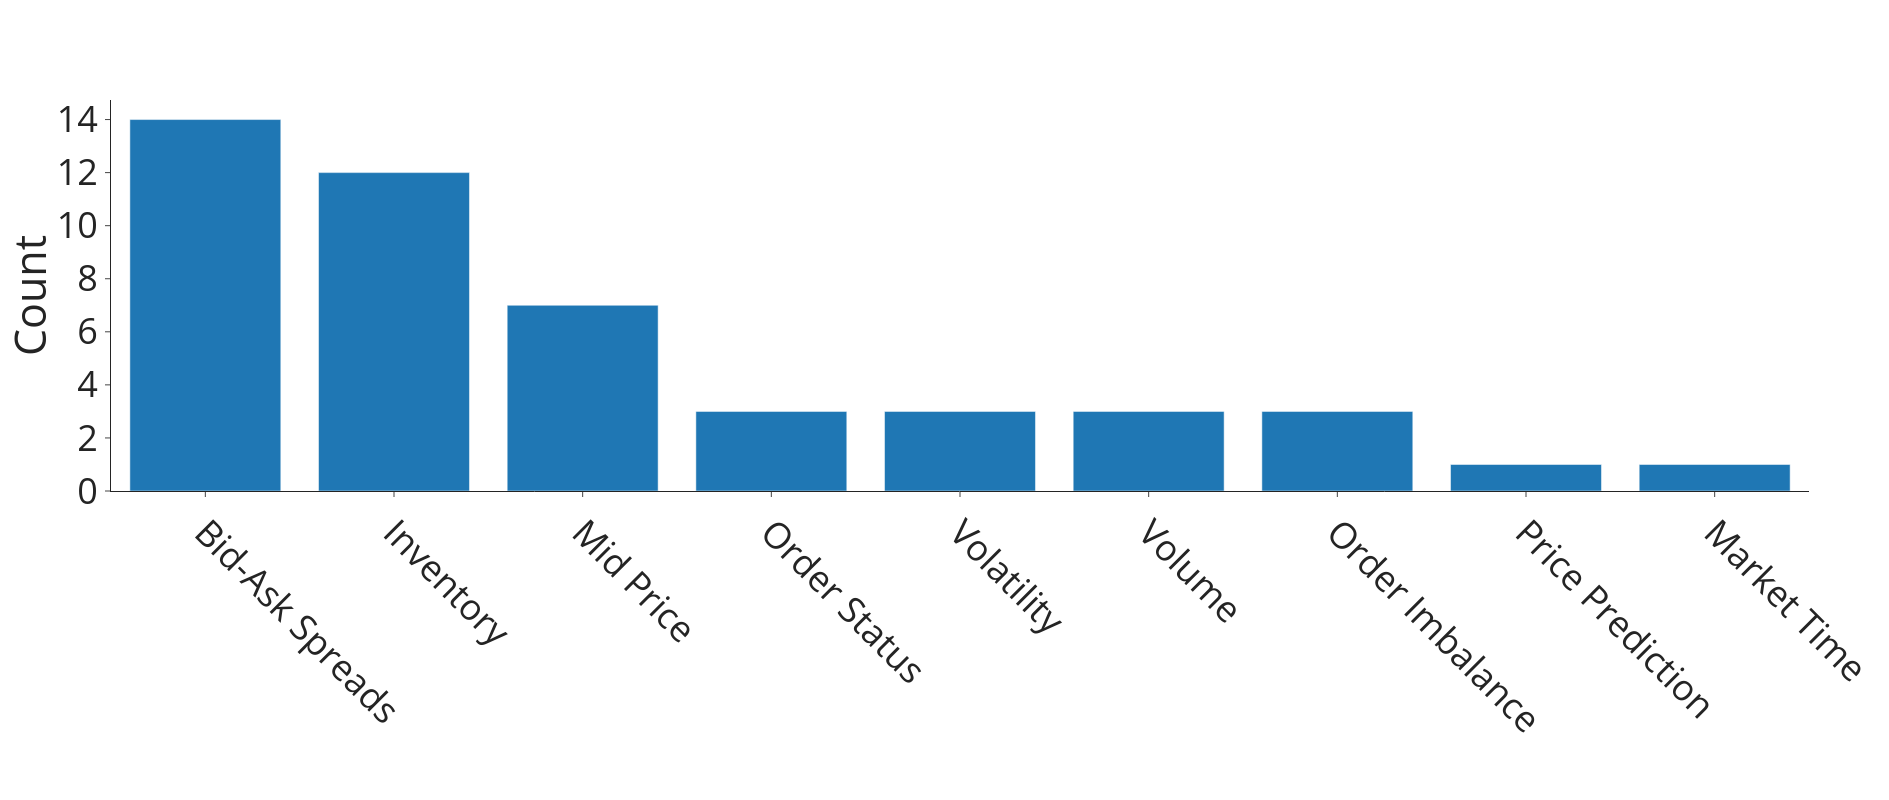
\includegraphics[width=0.8\textwidth]{images/state_space}
    \caption{State Space}
    \label{fig:state-space}
\end{figure}

% Choosen State Space
% State variable
% Total times used
%{
%    "inventory": "Agent inventory",
%    "bidask spread": "Bid-Ask spread",
%    "lob": "Price Levels",
%    "midprice": "Midprice",
%    "order status": "Posted order status",
%    "volume": "Transaction volume",
%    "order imbalance": "Order imbalance",
%    "volatility": "Volatility",
%    "price prediction": "Price prediction",
%    "time": "Market time"
%}